\documentclass[11pt]{article}
\usepackage[T1]{fontenc}
\usepackage{lmodern,amsmath,amssymb,graphicx,xcolor,booktabs,array,enumitem}
\usepackage[letterpaper,margin=0.78in]{geometry}
\usepackage[colorlinks=true,linkcolor=blue,urlcolor=teal]{hyperref}
\usepackage{fancyhdr}
\definecolor{ink}{HTML}{172C3B}
\definecolor{teal}{HTML}{087F82}
\definecolor{blue}{HTML}{265DAB}
\pagestyle{fancy}\fancyhf{}
\fancyhead[L]{\footnotesize OpenAI math: independent illustrated reading editions}
\fancyfoot[C]{\thepage}
\setlength{\headheight}{15pt}
\setlength{\parindent}{0pt}\setlength{\parskip}{7pt}
\setlength{\emergencystretch}{2em}
\hypersetup{pdfauthor={Independent explanatory edition prepared with OpenAI Codex}}
\begin{document}
\begin{center}{\LARGE\bfseries How can a matrix product require fewer multiplications?}\par\vspace{12pt}{\large An illustrated reader for the source's 9/4 exponent argument}\par\vspace{16pt}Independent reading edition, October 14, 2026\end{center}
\section*{Start here}A matrix is a rectangular table of numbers. Matrix multiplication combines each row of the first table with each column of the second. The familiar method performs about $n^3$ scalar multiplications for two $n\times n$ matrices, but algebraic identities can reuse intermediate products and reduce the asymptotic exponent.

The source claims an upper bound of $9/4$ over the complex numbers. Its route is indirect: encode bilinear computations as tensors, study numerical invariants called characters, derive inequalities for polynomial multiplication, and use those inequalities to constrain matrix multiplication.

This is not a benchmark report or an implementation ready to replace a numerical library. The theorem is in an arithmetic-operation model, and its asymptotic algorithm can have constants depending on a desired accuracy in the exponent. The figures focus on actual coefficient arrays and the finite separation mechanism, then explain the final growth comparison.
\paragraph{Reading prerequisites.} Ordinary arithmetic is enough for the opening examples. Later chapters introduce the specialized vocabulary; checking every original proof requires additional study.\par\textbf{Attribution.} Original manuscript by OpenAI. Added explanations and figures prepared with OpenAI Codex. This is not an official revision or independent theorem validation.\par\href{https://github.com/openai/math/tree/1581d4cbdd69a0faf34b2089614fe2a814316a6a/preprints/Matrix-Multiplication-Nine-Fourths-October-2-2026}{Pinned original manuscript and citation}.\newpage\section*{The source claim, precisely}Theorem 1.1 states that for every $\varepsilon>0$, two $n\times n$ complex matrices can be multiplied in $O_\varepsilon(n^{9/4+\varepsilon})$ scalar arithmetic operations. Equivalently, the source claims $\omega\le9/4$. It does not assert a practical finite-size crossover, a bit-complexity bound of that form, or a competitive floating-point implementation.\paragraph{How to read this edition.} Each chapter gives one concrete illustration, then explains how it connects to the source. Captions identify toys and original constructions. Source anchors use the original manuscript\textquotesingle s section and page numbering. The expanded PDF places this guide before the complete unchanged original PDF, preserving the original page numbers and bibliography.\subsection*{Your route through the argument}\begin{enumerate}\item Every output entry is a row-column dot product
\item Polynomial multiplication has a concrete coefficient pattern
\item Shared variables prevent a full direct sum
\item A Fourier filter and a square enforce matching labels
\item The three sectors are visible in the support
\item Compare forced growth with an interpolation ceiling
\end{enumerate}\paragraph{Verification scope.} The accompanying code checks the displayed finite examples and preserves original-file hashes. These checks do not replace the analytic, algebraic, asymptotic, or formal proof obligations in the source.\newpage\section*{Every output entry is a row-column dot product}
\begin{center}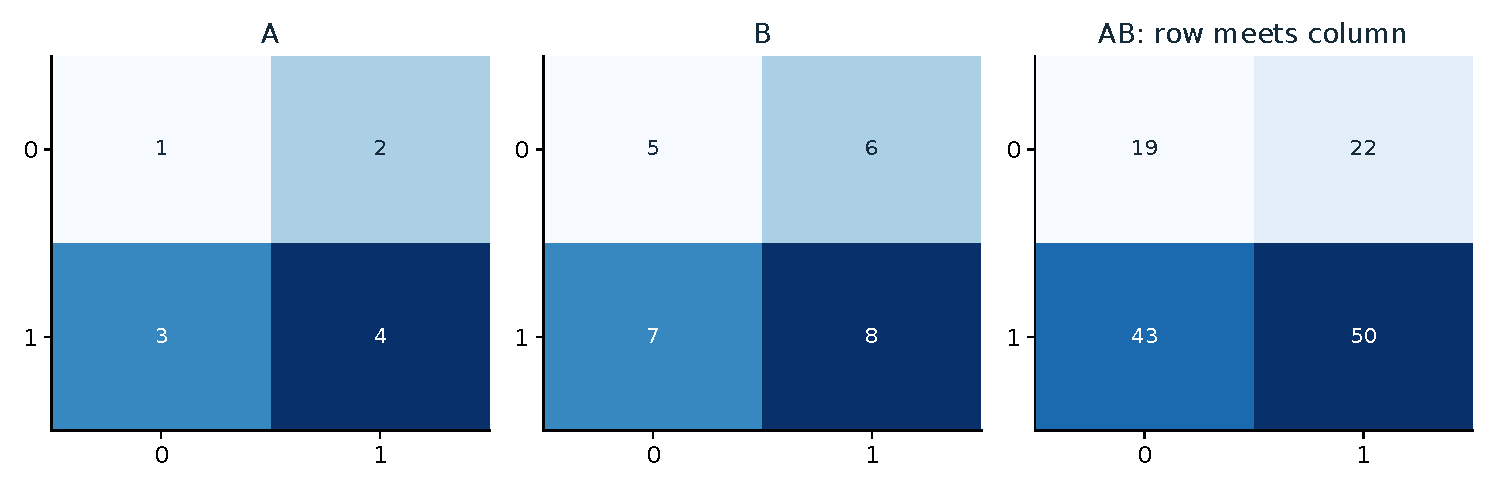
\includegraphics[width=\linewidth,height=2.35in,keepaspectratio]{figures/01-product.pdf}\end{center}
{\small\color{teal}\textbf{Figure 1.} The displayed product is [[19,22],[43,50]]. For example, its upper-left entry is 1$\times$5+2$\times$7=19, not the entrywise product 1$\times$5.\par}
To compute one output entry, multiply matching entries of a row and column and add. For the upper-left entry, $(1,2)$ meets $(5,7)$, giving nineteen. The other three entries are $1\cdot6+2\cdot8=22$, $3\cdot5+4\cdot7=43$, and $3\cdot6+4\cdot8=50$.

For $n\times n$ matrices, there are $n^2$ outputs and $n$ products per output, so this direct method uses $n^3$ scalar multiplications. Faster algebraic algorithms change the organization of the calculation rather than the meaning of the result.

A bilinear algorithm first forms linear combinations of the first input and of the second input, multiplies selected pairs of those combinations, then combines the results linearly. A tensor records the coefficients of such a bilinear map. For matrix multiplication the trilinear form is $\sum_{i,j,k}x_{ij}y_{jk}z_{ki}$, where the third variable group records the output pairing.

The three variable groups are called legs. They are not spatial axes or three stages of execution. Keeping track of which variables belong to each leg is essential when combining or separating computations.
{\footnotesize\color{blue}\textbf{Source anchor:} Sections 1-2: arithmetic exponent, tensors, and equation (2.2).\par}
\newpage\section*{Polynomial multiplication has a concrete coefficient pattern}
\begin{center}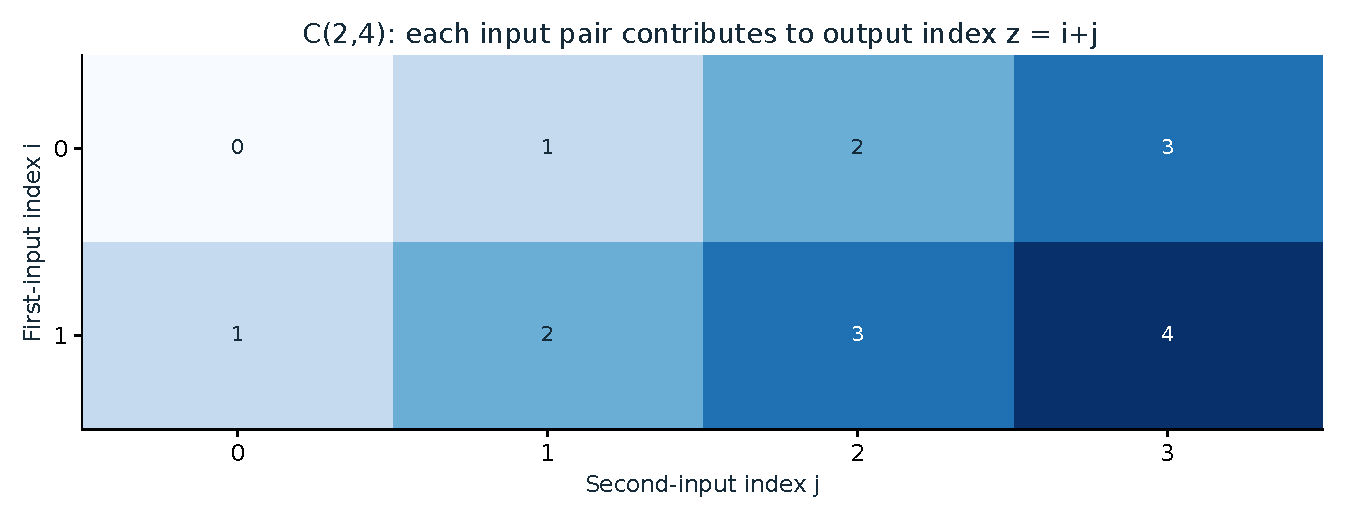
\includegraphics[width=\linewidth,height=2.35in,keepaspectratio]{figures/02-polynomial.pdf}\end{center}
{\small\color{teal}\textbf{Figure 2.} The C(2,4) array has eight input products. A cell (i,j) contributes to output coefficient i+j, producing output indices 0 through 4.\par}
Multiply a polynomial with two coefficients by one with four coefficients. Each first-input coefficient $x_i$ multiplies each second-input coefficient $y_j$, and the result contributes to coefficient $i+j$:
\[C(2,4)=\sum_{i=0}^{1}\sum_{j=0}^{3}x_i y_j z_{i+j}.\]
The table shows exactly which output coordinate receives each product. Equal numbers lie along the relevant anti-diagonals.

For general input lengths $a,b$, the output length is $a+b-1$. Evaluating both polynomials at that many distinct points, multiplying the values, and interpolating gives a rank upper bound of $a+b-1$. The source uses the output flattening to match it with a lower bound, hence $R(C(a,b))=a+b-1$.

Tensor rank is the smallest number of simple bilinear products needed to represent the map, after allowing linear combinations of inputs and outputs. This ordinary tensor rank is not the matrix-multiplication exponent. Its role is to bound the character values of a convenient test family. A character is normalized, additive on full direct sums, multiplicative on tensor products, and monotone under restrictions.

Those properties make characters useful numerical witnesses, but a detecting-character theorem is also needed to connect bounds on all such witnesses back to the matrix-multiplication problem.
{\footnotesize\color{blue}\textbf{Source anchor:} Section 4, equations (4.1)-(4.5); Lemma 2.2.\par}
\newpage\section*{Shared variables prevent a full direct sum}
\begin{center}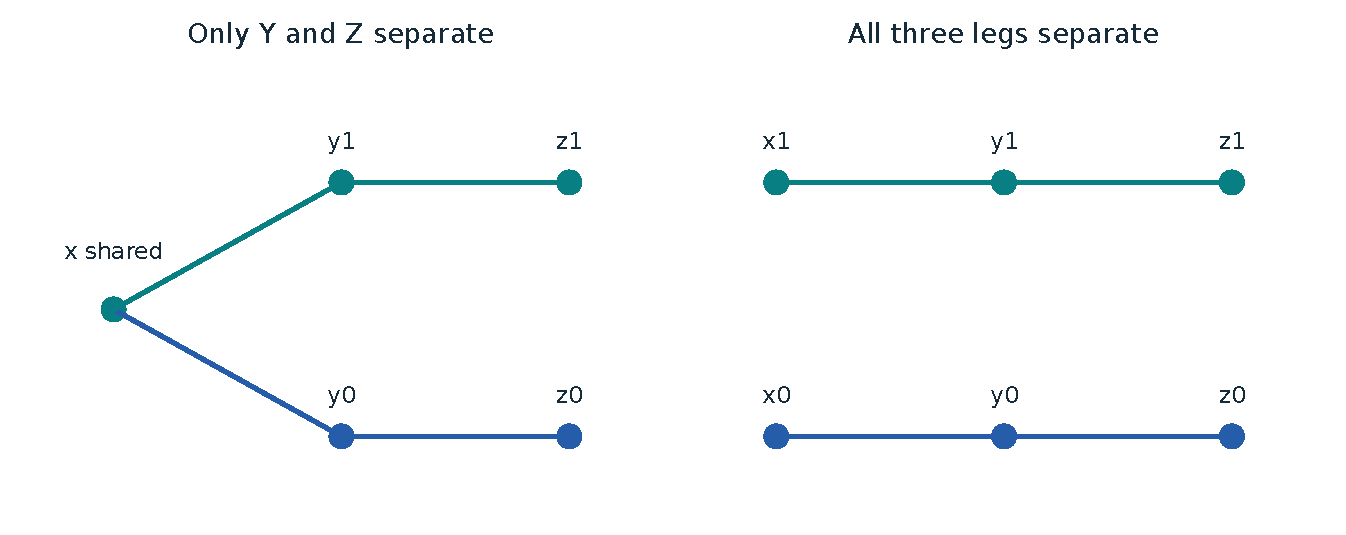
\includegraphics[width=\linewidth,height=2.35in,keepaspectratio]{figures/03-shared-leg.pdf}\end{center}
{\small\color{teal}\textbf{Figure 3.} Left: x·y$_0$z$_0$+x·y$_1$z$_1$ shares its X variable. Right: x$_0$y$_0$z$_0$+x$_1$y$_1$z$_1$ uses independent variables on all three legs. These are different tensors.\par}
Suppose two useful blocks already have separate second-input and output variables but share the first-input space. They cannot yet be treated as a full direct sum. In a full direct sum, every block has its own variables on every leg.

The left illustration has one common $x$. Relabeling it $x_0$ in one term and $x_1$ in the other would grant an extra independent input without paying for it. It is not a free change of notation. Tensor constructions must implement such separation through legal linear substitutions, copies, and degenerations.

Proposition 3.1 begins with $M$ sectors sharing their first leg. It uses $5M$ copies of the input tensor and produces $M$ fully independent blocks, each carrying an additional $M$-dimensional dot product. The source counts both the copies used and the auxiliary factor retained.

The extra dot-product dimension is not another collection of independent direct-sum blocks. Confusing these multiplicities would overstate the construction's gain. In tensor powers, the balance between the number of sectors and this retained factor yields the entropy inequality used later.
{\footnotesize\color{blue}\textbf{Source anchor:} Proposition 3.1 and Corollary 3.2.\par}
\newpage\section*{A Fourier filter and a square enforce matching labels}
\begin{center}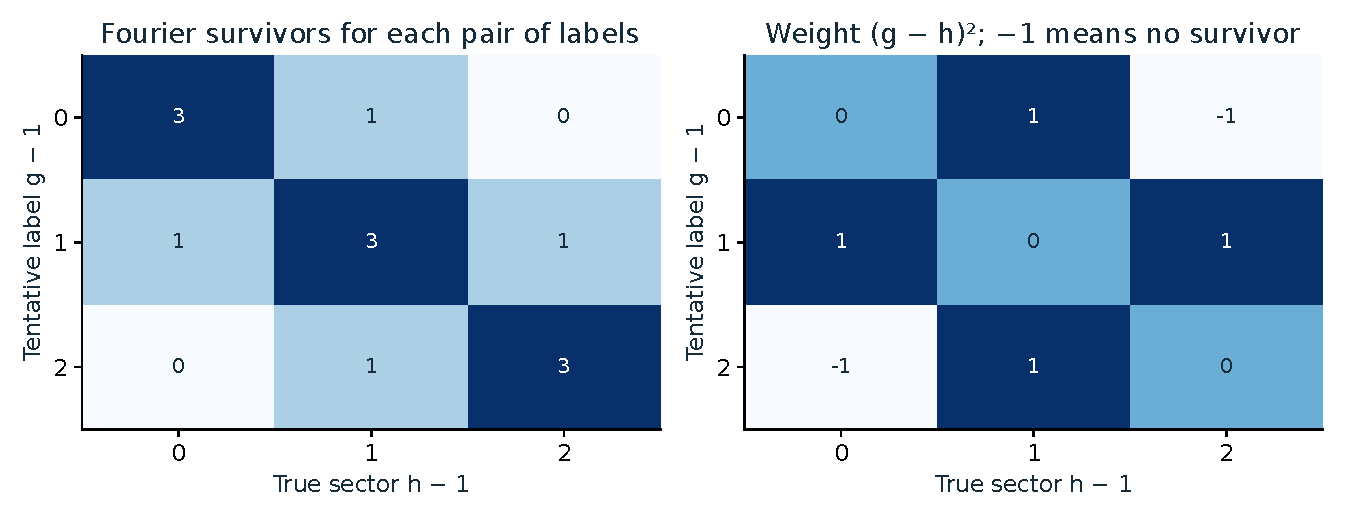
\includegraphics[width=\linewidth,height=2.35in,keepaspectratio]{figures/04-separation.pdf}\end{center}
{\small\color{teal}\textbf{Figure 4.} For M=3, the left table counts tuples surviving u$-$v+2(g$-$h)=0. Surviving terms have weight (g$-$h)$^2$; weight zero requires g=h and then u=v.\par}
The finite construction gives the shared leg a tentative sector label $g$, while the other legs know the true sector $h$. Auxiliary indices $u,v$ run from one to $M$. Summing phases over $L=5M$ roots of unity kills all terms except those satisfying
\[u-v+2(g-h)=0.\]
The index range is smaller than $L$, so equality modulo $L$ here means actual integer equality, not an accidental wraparound.

Next the source gives the three legs weights $g^2$, $hu-h^2$, and $-hv$. On a surviving term their sum is
\[g^2+hu-h^2-hv=(g-h)^2.\]
It is nonnegative, and its minimum zero occurs exactly when the tentative and true labels agree. The filter then also forces $u=v$, leaving the desired dot product.

The script exhaustively enumerates all $3^4$ index tuples in this example and checks the identity and zero-weight condition. It does not numerically approximate roots of unity to decide equality.

This finite calculation illustrates the proposition. Its asymptotic use also requires the source's interpolation passage from degenerations to character inequalities and its tensor-power counting argument.
{\footnotesize\color{blue}\textbf{Source anchor:} Proposition 3.1 and Lemma 2.3.\par}
\newpage\section*{The three sectors are visible in the support}
\begin{center}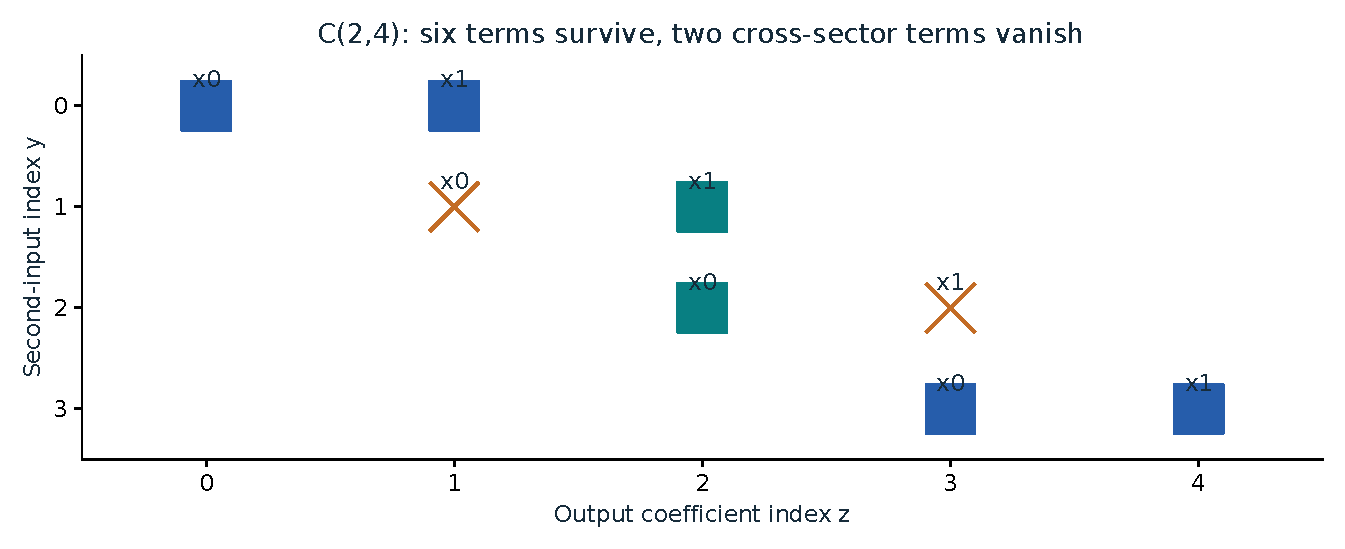
\includegraphics[width=\linewidth,height=2.35in,keepaspectratio]{figures/05-sectors.pdf}\end{center}
{\small\color{teal}\textbf{Figure 5.} For a=2 and h=1, the source's shifted-tripling construction uses C(2,4). Two supported terms receive weight +1 and vanish; six remain in three matched sectors.\par}
A supported term satisfies $z=x+y$. In this example, the left second-input sector is $y=0$, the middle is $y=1,2$, and the right is $y=3$. The corresponding output sectors are $z=0,1$, then $z=2$, then $z=3,4$.

Give weight $+1$ to middle $Y$ coordinates, weight $-1$ to middle $Z$ coordinates, and zero elsewhere. The term $x_0y_1z_1$ has weight one, as does $x_1y_2z_3$. They disappear in the minimum-weight degeneration. Every other supported term has weight zero; none has negative total weight.

The surviving outer blocks have the shape $C(2,1)$. The middle has exchanged second and third legs and a reversed first-leg basis. This individual-branch identification is not permission to apply incompatible first-leg maps to the shared input of the whole tensor.

The paper combines all six permutations of the legs in a symmetrized character profile. Permutation factors then balance correctly, yielding $P(a,3h+a-1)\ge3P(a,h)$. The little support diagram explains the finite sectors; the profile inequality also uses the shared-leg entropy result.
{\footnotesize\color{blue}\textbf{Source anchor:} Lemma 4.2 and original Figure 1.\par}
\newpage\section*{Compare forced growth with an interpolation ceiling}
\begin{center}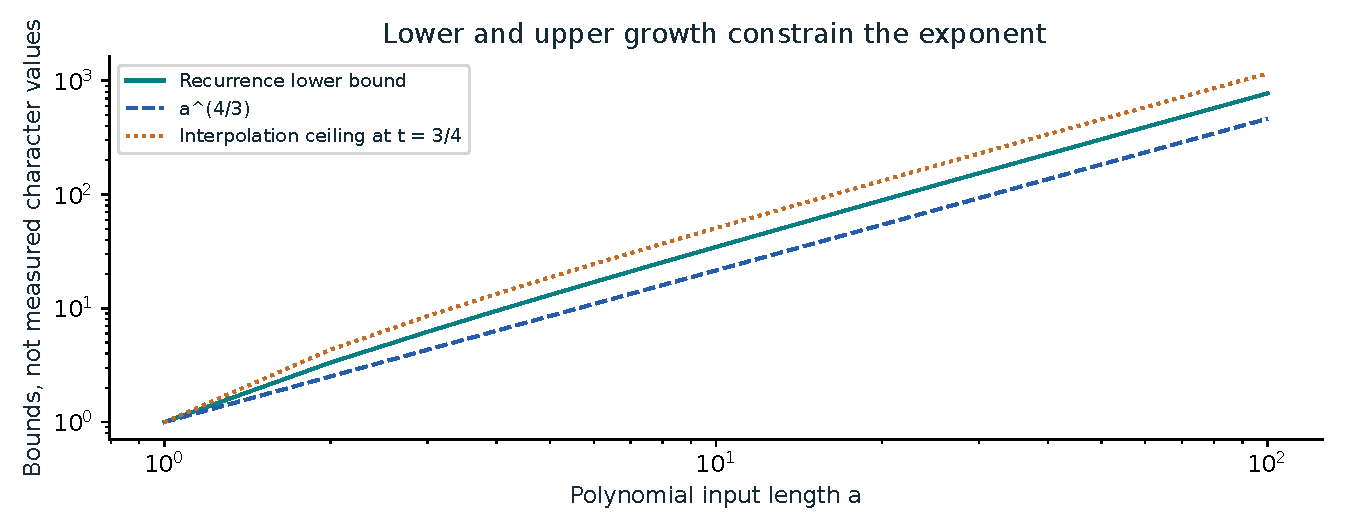
\includegraphics[width=\linewidth,height=2.35in,keepaspectratio]{figures/06-growth.pdf}\end{center}
{\small\color{teal}\textbf{Figure 6.} The curves show bounds from the discrete growth argument, not sampled values of an unknown tensor character. At t=3/4, the interpolation ceiling has the same asymptotic power 4/3.\par}
The source defines a positive symmetric profile $P(a,b)$ from all six permuted character values. It has boundary $P(1,b)=b$, concave successive increments in each variable, and the shifted-tripling inequality. Together these imply $P(a,a)\ge a^{4/3}$.

One intermediate sequence satisfies $H_1=1$ and
\[H_a\ge\prod_{m=1}^{a-1}\left(1+\frac1{3m}\right).\]
Cubing each factor bounds it below by $1+1/m$, whose product telescopes to $a$. The script checks this finite product inequality exactly over the plotted range. The source proves it for every positive integer.

Interpolation separately gives $P(a,a)\le(2a-1)^{1/t}$. If $t>3/4$, its exponent $1/t$ would be smaller than $4/3$, eventually contradicting the lower bound. Thus $t\le3/4$, giving character values on matrix multiplication at most $n^{9/4}$.

The detecting-character argument then bounds exact-rank exponents. Finally, a fixed rank decomposition is recursively applied to matrix blocks, with padding for arbitrary sizes and an arbitrarily small exponent allowance. These last bridges are essential: a favorable plot of an abstract profile does not itself provide an algorithm or prove the headline theorem.
{\footnotesize\color{blue}\textbf{Source anchor:} Lemma 5.1, Theorem 1.1 proof, and Appendix A.\par}
\newpage\section*{A vocabulary you can return to}
\paragraph{Bilinear map}Linear in either input when the other input is fixed.
\paragraph{Tensor leg}One of the three variable groups in a trilinear encoding.
\paragraph{Full direct sum}Independent variables for each component on all three legs.
\paragraph{Degeneration}Retain minimum-weight terms after parameterized substitutions.
\paragraph{Character}A normalized additive, multiplicative, restriction-monotone tensor invariant.
\paragraph{Arithmetic exponent}An asymptotic power counting scalar operations, with arbitrary positive exponent slack.
\section*{What this edition checks}The guide checks its numerical matrix product, finite Fourier-label conditions, three-sector support, and finite product inequalities. It does not independently prove the shared-leg construction for every tensor, the determinant-filtration lemma, spectral separation, or the source's final algorithmic claim. The separate matrix-sector refinement repository studies an abstract obstruction with its own hypotheses; it is not substituted for this newer manuscript's argument.
\paragraph{A useful self-test.} Explain what each plotted quantity counts, which examples are illustrative, and where the source needs a statement for every input or every sufficiently large size. If a picture seems to establish the full theorem by itself, revisit its caption and source anchor.\paragraph{Sources and reuse.}\href{https://github.com/openai/math/tree/1581d4cbdd69a0faf34b2089614fe2a814316a6a/preprints/Matrix-Multiplication-Nine-Fourths-October-2-2026}{An Upper Bound of 9/4 for the Matrix Multiplication Exponent}, OpenAI. Original bibliography and manuscript-specific citation are included with the source. Source snapshot: \texttt{1581d4cbdd69}. This derivative is distributed under Apache-2.0 with the original attribution; see the repository LICENSE and NOTICE.\end{document}